
\chapter{RL Training and Policy Selection}
\label{app:rl_training}

\section{PPO Configuration}

Table~\ref{tab:ppo_specifications} records the PPO backbone settings used for navigation-policy training. The curriculum increases task difficulty while the optimization configuration remains fixed. GAE denotes generalized advantage estimation; its $\lambda$ parameter is distinct from the multiplier used by PPO-Lagrangian.

\begin{table}[H]
\centering
\caption{PPO backbone and training budget.}
\label{tab:ppo_specifications}
{\small\renewcommand{\arraystretch}{1.15}
\begin{tabularx}{\linewidth}{@{}Yl@{}}
\toprule
\textbf{Hyperparameter} & \textbf{Value}\\
\midrule
Hidden layers & $64,\;64$ units\\
Learning rate & $3\times10^{-4}$\\
Discount factor $\gamma$ & $0.99$\\
GAE parameter $\lambda$ & $0.95$\\
PPO clipping ratio & $0.20$\\
Entropy coefficient & $0.005$\\
Value-loss coefficient & $0.50$\\
Initial action log standard deviation & $-0.50$\\
Maximum gradient norm & $1.0$\\
Optimization epochs per update & $10$\\
Minibatches per epoch & $8$\\
Parallel environments & $4096$\\
Rollout length per environment & $258$ steps\\
Transitions per update & $1{,}056{,}768$\\
Training updates & $100$\\
Training transitions & $105{,}676{,}800$\\
Environment time step & $0.05$\,s\\
Training hardware & NVIDIA A100\\
\bottomrule
\end{tabularx}}
\end{table}

The interaction budget is aggregated across all parallel training environments.

\clearpage
\section{Policy-Selection Ablation}

The policy-selection study considers five RL regimes with five random seeds per regime, for 25 training runs. The comparison separates the effect of CBF action filtering from Lagrangian constraint handling and adversarial training.

\begin{table}[H]
\centering
\caption{RL regimes considered in the policy-selection study.}
\label{tab:rl_regimes}
{\small\renewcommand{\arraystretch}{1.35}
\begin{tabularx}{\linewidth}{@{}p{.37\linewidth}Yc@{}}
\toprule
\textbf{Regime} & \textbf{Training mechanism} & \textbf{Seeds}\\
\midrule
PPO & Reward-driven policy learning & 5\\
PPO+CBF & CBF correction of executed actions & 5\\
PPO-Lagrangian & Policy learning with a constraint multiplier & 5\\
PPO-Lagrangian+CBF & Constraint multiplier and CBF action filtering & 5\\
PPO+CBF+Adversarial & CBF filtering with an adversarial disturbance policy & 5\\
\bottomrule
\end{tabularx}}
\end{table}

\begin{figure}[H]
\centering
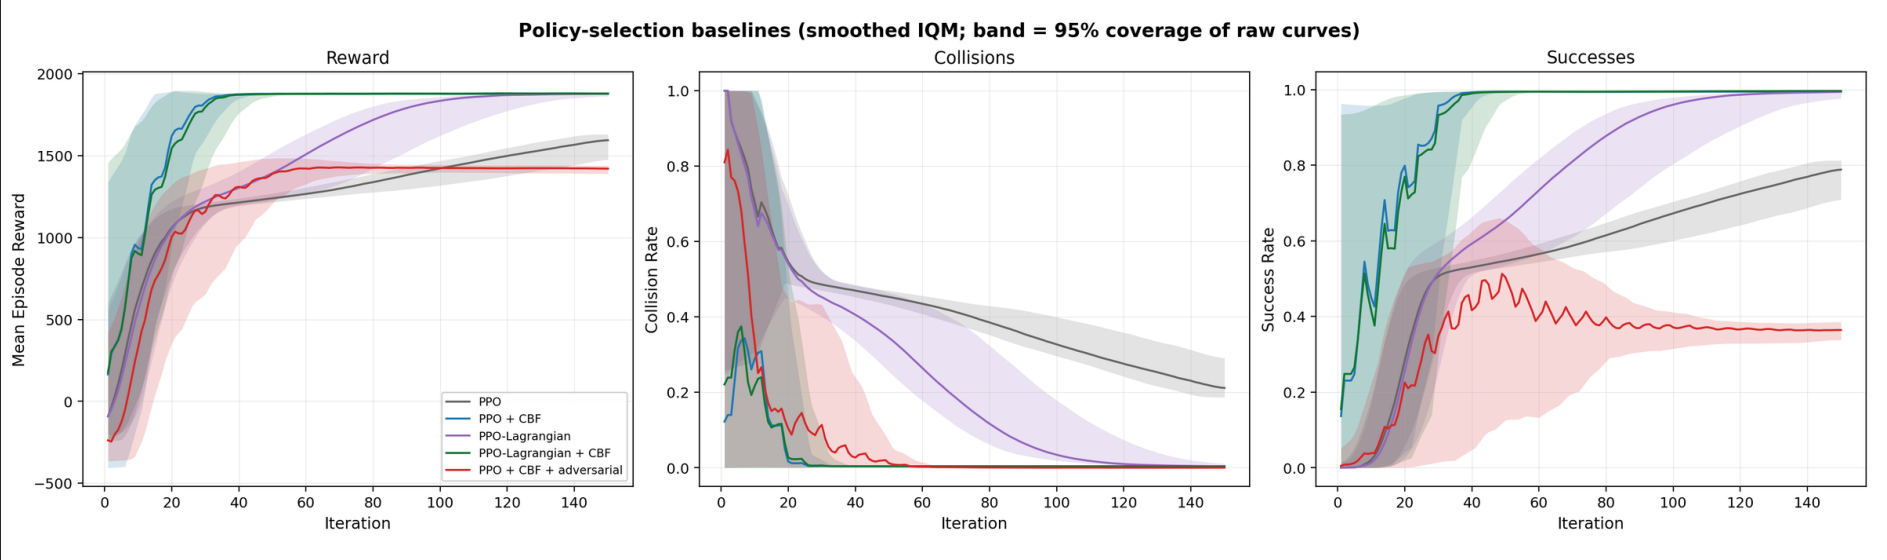
\includegraphics[width=\linewidth]{figures/rl_ablation_training.png}
\caption[Five-regime policy-selection training curves]{Reward, collision rate and success rate across the five RL regimes. Curves show the smoothed interquartile mean (IQM); shaded bands indicate 95\% coverage of raw curves, not confidence intervals.}
\label{fig:rl_ablation_training}
\end{figure}

Figure~\ref{fig:rl_ablation_training} shows that PPO+CBF and PPO-Lagrangian+CBF both reach high success and low collision rates early. PPO+CBF was retained for this favorable balance of learning efficiency and safety, with a simpler training objective that avoids multiplier updates and adversary optimization.

Learning efficiency here refers to progress over training interactions. The selected policy remains fixed in the main benchmark, where our contribution is the online adaptation of its downstream safety margin.
